% HW3 high dimensional data

\documentclass[12pt, leqno]{article}
\usepackage{amsfonts, amsmath, amssymb}
\usepackage{amsthm}
\usepackage{mathtools}
\usepackage{fancyhdr}
\usepackage{hyperref}
\usepackage{graphicx}
\usepackage{caption}
\usepackage{subcaption}
\usepackage{float}
\usepackage{mathrsfs}
\usepackage{array} 
\usepackage{rotating}
\usepackage{rotating}
\usepackage{booktabs}
\usepackage{bbm}
%\usepackage{babel}
\providecommand{\abs}[1]{\lvert#1\rvert}
\providecommand{\norm}[1]{\lVert#1\rVert}
\newcommand{\macheps}{\epsilon_{\mbox{\scriptsize mach}}}
\let\oldhat\hat
\renewcommand{\vec}[1]{\mathbf{#1}}
\renewcommand{\hat}[1]{\oldhat{{#1}}}
\def\rp{\ensuremath \mathbb{R}^p}
\def\rpp{\ensuremath \mathbb{R}^{p \times p}}
\def\s{\ensuremath\Sigma}
\def\om{\ensuremath\Omega}
\def\pd{\ensuremath\mathbb{P}^+}
\def\pg{\ensuremath\mathbb{P}_{{G}}}
\def\E{\ensuremath\mathbb{E}}
\def\normdist[#1]#2{\ensuremath \sim \mathcal{N} (#1,#2) }
\def\ndist1{\ensuremath \sim \mathcal{N}  (\mu, \sigma)}
\def\ndistvec{\ensuremath \sim \mathcal{N}_p ( {\mu},  {\Sigma})}
\def\lra{\ensuremath\Leftrightarrow}
\def\stackrel#1#2{\mathrel{\mathop{#2}\limits^{#1}}}
\newcommand\ind{\protect\mathpalette{\protect\independenT}{\perp}}
\def\independenT#1#2{\mathrel{\rlap{$#1#2$}\mkern2mu{#1#2}}}
\makeatletter
\newtheorem{thm}{Theorem}[]
\newtheorem{lemma}{Lemma}[]
\newtheorem{defn}[thm]{Definition}
\newcommand{\sign}{\mathrm{sign}}
\newcommand{\distas}[1]{\mathbin{\overset{#1}{\kern\z@\sim}}}%
\newsavebox{\mybox}\newsavebox{\mysim}
\newcommand{\dist}[1]{%
  \savebox{\mybox}{\hbox{\kern3pt$\scriptstyle#1$\kern3pt}}%
  \savebox{\mysim}{\hbox{$\sim$}}%
  \mathbin{\overset{#1}{\kern\z@\resizebox{\wd\mybox}{\ht\mysim}{$\sim$}}}%
}
\makeatother

\begin{document}
\pagestyle{fancy}
\lhead{Syed Rahman}
\rhead{STA6707}

\begin{center}
{\large {\bf Homework 3 Partial Solutions}}
\end{center}

\paragraph{Part 1:} For this problem, I was looked for the basic
clustering and some comparison across a range of k. I tried k from 2
through 10. The average silhouette plots are included below. The
average silhouette scores for each plot are shown below. In addition,
the last row shows the average over all clusters. In most cases, k =
2, seems to give the best results.

\begin{figure}
\centering
\begin{subfigure}{.5\textwidth}
  \centering
  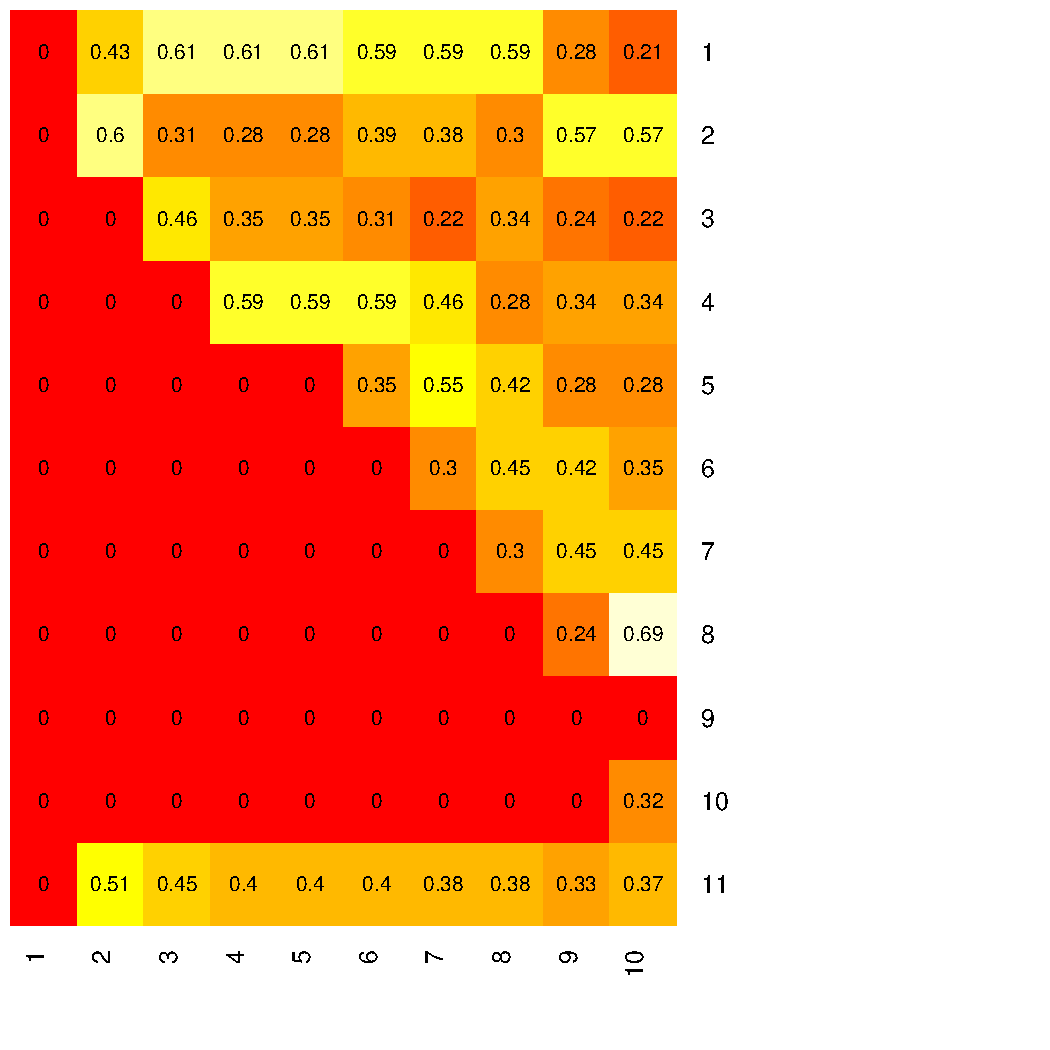
\includegraphics[width=.65\linewidth]{hclsil.pdf}
  \caption{Hierarchical Clustering}
  \label{fig:sub1}
\end{subfigure}%
\begin{subfigure}{.5\textwidth}
  \centering
  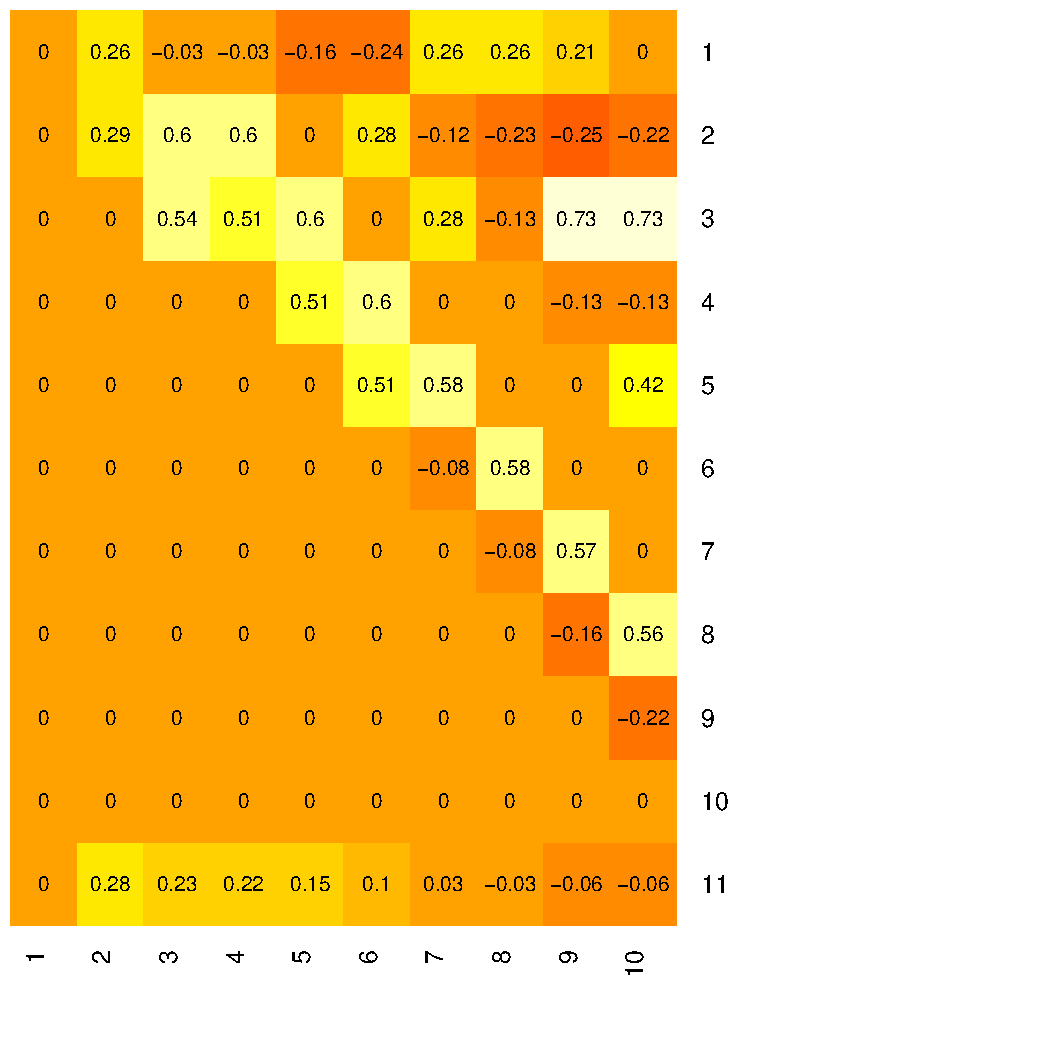
\includegraphics[width=.65\linewidth]{agnessil.pdf}
  \caption{Agglomerative Clustering}
  \label{fig:sub2}
\end{subfigure}
\caption{Average Silhoutte Plots}
\label{fig1}
\end{figure}

\begin{figure}
\centering
\begin{subfigure}{.5\textwidth}
  \centering
  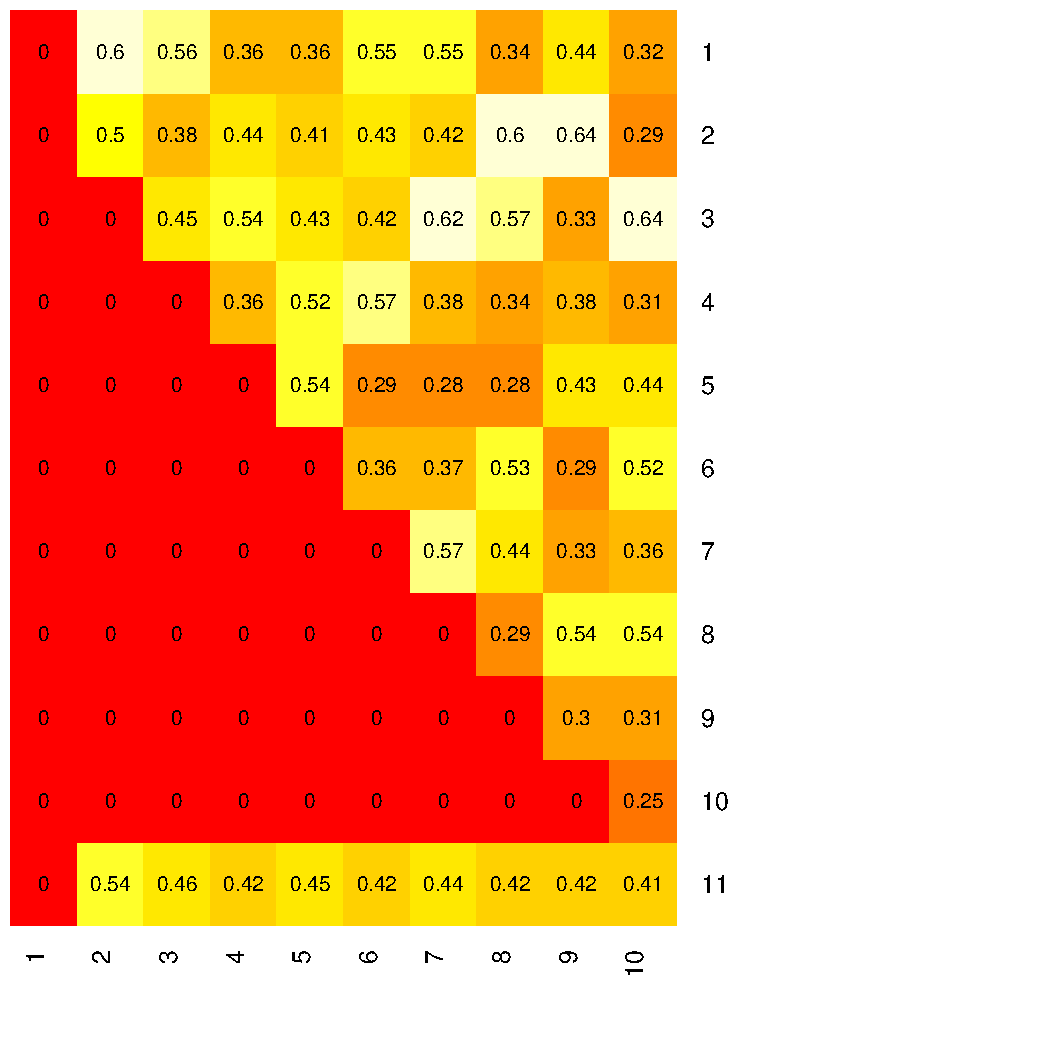
\includegraphics[width=.65\linewidth]{kmeanssil.pdf}
  \caption{K-means Clustering}
  \label{fig:sub3}
\end{subfigure}%
\begin{subfigure}{.5\textwidth}
  \centering
  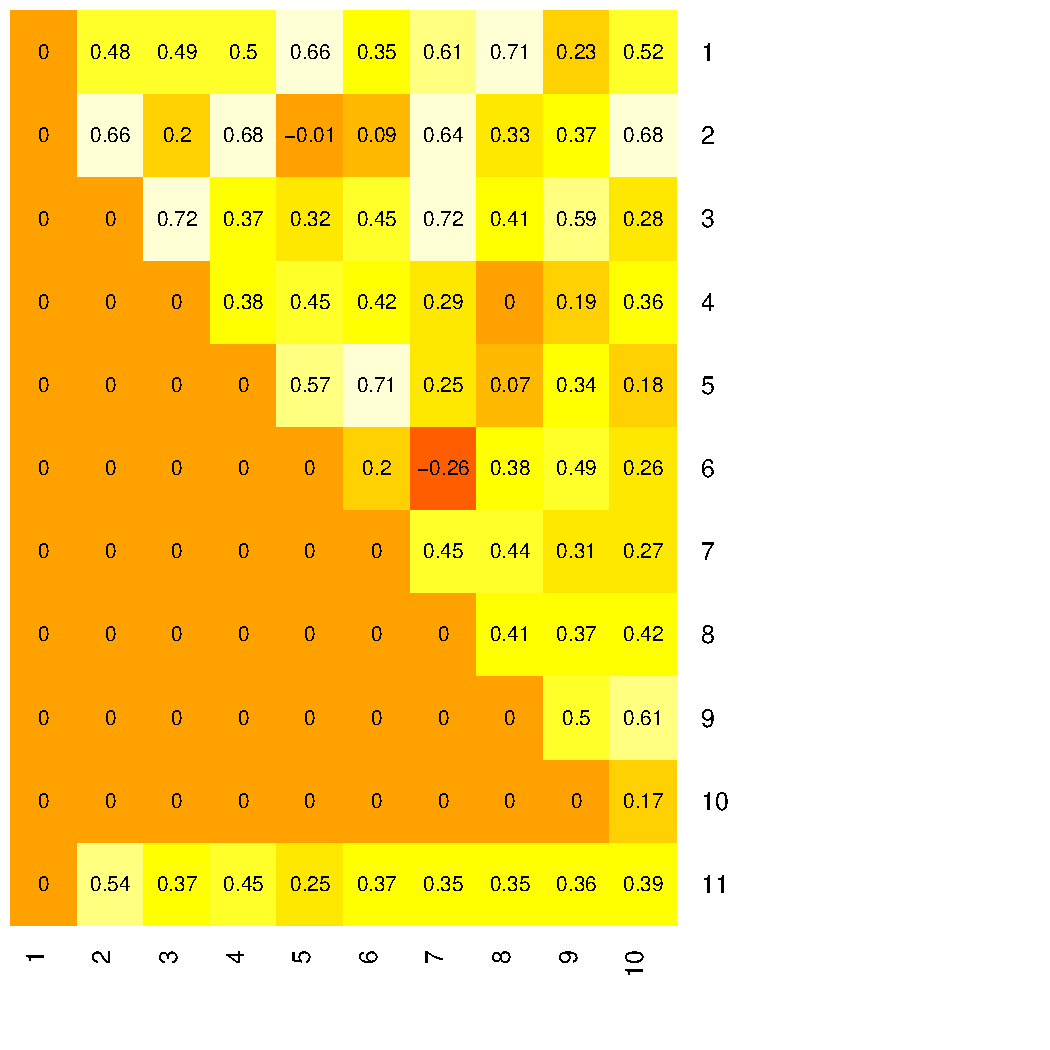
\includegraphics[width=.65\linewidth]{specsil.pdf}
  \caption{Spectral Clustering}
  \label{fig:sub4}
\end{subfigure}
\caption{Average Silhoutte Plots}
\label{fig1}
\end{figure}

\newpage
\paragraph{Part 2:} The confusion matrix for clusters versus area and
clusters versus region are show below. We use spectral clustering as
the performance was pretty good for that. In general, it seems like
the clustering is decent when compared to the real data, but there
isn't $100\%$ accuracy. In the first case, 279 from Area 1 gets
put in cluster 1, while in the second table, 223 from Area 1 gets put
in cluster 3 and so on.
\begin{table}[ht]
\centering
\begin{tabular}{rrrr}
  \hline
Cluster/Area & 1 & 2 & 3 \\ 
  \hline
1 & 279 &  98 &   4 \\ 
  2 &  44 &   0 & 147 \\ 
   \hline
\end{tabular}
\end{table}

% latex table generated in R 3.2.4 by xtable 1.8-2 package
% Tue Apr 19 13:30:29 2016
\begin{table}[ht]
\centering
\begin{tabular}{rrrr}
  \hline
Cluster/Area & 1 & 2 & 3 \\ 
  \hline
1 &  56 &  71 &  10 \\ 
  2 &  44 &   0 & 141 \\ 
  3 & 223 &  27 &   0 \\ 
   \hline
\end{tabular}
\end{table}

\begin{table}[ht]
\centering
\begin{tabular}{rrrr}
  \hline
Cluster/Area & 1 & 2 & 3 \\ 
  \hline
1 & 195 &  18 &   0 \\ 
  2 &   3 &  80 &  12 \\ 
  3 &  87 &   0 &  11 \\ 
  4 &  38 &   0 & 128 \\ 
   \hline
\end{tabular}
\end{table}

\begin{table}[ht]
\centering
\begin{tabular}{rrrrrrrrrr}
  \hline
Cluster/Region & 1 & 2 & 3 & 4 & 5 & 6 & 7 & 8 & 9 \\ 
  \hline
1 &   0 &   0 &   1 &   0 &  65 &   0 &   0 &   0 &   0 \\ 
  2 &  12 &   0 &   0 &   1 &   0 &   0 &  23 &   2 &  51 \\ 
  3 &   0 &   0 &  11 &   1 &   0 &   0 &   0 &   0 &   0 \\ 
  4 &   0 &   0 &   1 &   0 &   0 &  33 &   0 &   0 &   0 \\ 
  5 &  13 &  55 &  15 &  26 &   0 &   0 &  27 &  48 &   0 \\ 
  6 &   0 &   1 & 178 &   8 &   0 &   0 &   0 &   0 &   0 \\ 
   \hline
\end{tabular}
\end{table}

% latex table generated in R 3.2.4 by xtable 1.8-2 package
% Tue Apr 19 13:33:14 2016
\begin{table}[ht]
\centering
\begin{tabular}{rrrrrrrrrr}
  \hline
Cluster/Region & 1 & 2 & 3 & 4 & 5 & 6 & 7 & 8 & 9 \\ 
  \hline
1 &   1 &  51 &  15 &  13 &   0 &   0 &   2 &   1 &   0 \\ 
  2 &   0 &   0 &   1 &   0 &  65 &   0 &   0 &   2 &   0 \\ 
  3 &   0 &   0 &  29 &   1 &   0 &   0 &   0 &   0 &   0 \\ 
  4 &   0 &   1 & 157 &   8 &   0 &   0 &   0 &   0 &   0 \\ 
  5 &   0 &   0 &   4 &   0 &   0 &  33 &   0 &   0 &   0 \\ 
  6 &  14 &   4 &   0 &  14 &   0 &   0 &  35 &  46 &   0 \\ 
  7 &  10 &   0 &   0 &   0 &   0 &   0 &  13 &   1 &  51 \\ 
   \hline
\end{tabular}
\end{table}

\begin{table}[ht]
\centering
\begin{tabular}{rrrrrrrrrr}
  \hline
Cluster/Region & 1 & 2 & 3 & 4 & 5 & 6 & 7 & 8 & 9 \\ 
  \hline
1 &  15 &   4 &   0 &  12 &   0 &   0 &  34 &  47 &   0 \\ 
  2 &   0 &   0 & 149 &   4 &   0 &   0 &   0 &   0 &   0 \\ 
  3 &   1 &  51 &  15 &  13 &   0 &   0 &   3 &   1 &   0 \\ 
  4 &   0 &   1 &  28 &   4 &   0 &   0 &   0 &   0 &   0 \\ 
  5 &   0 &   0 &   1 &   0 &  65 &   0 &   0 &   1 &   0 \\ 
  6 &   9 &   0 &   0 &   0 &   0 &   0 &  13 &   1 &  51 \\ 
  7 &   0 &   0 &   1 &   0 &   0 &  33 &   0 &   0 &   0 \\ 
  8 &   0 &   0 &  12 &   3 &   0 &   0 &   0 &   0 &   0 \\ 
   \hline
\end{tabular}
\end{table}

\begin{table}[ht]
\centering
\begin{tabular}{rrrrrrrrrr}
  \hline
Cluster/Region  & 1 & 2 & 3 & 4 & 5 & 6 & 7 & 8 & 9 \\ 
  \hline
1 &   0 &   0 &  54 &   1 &   0 &   0 &   0 &   0 &   0 \\ 
  2 &  10 &   0 &   0 &   1 &   0 &   0 &  11 &   1 &  51 \\ 
  3 &   0 &   0 &  41 &   2 &   0 &   0 &   0 &   0 &   0 \\ 
  4 &  12 &   5 &   0 &   9 &   0 &   0 &  37 &   8 &   0 \\ 
  5 &   0 &   1 &  88 &   6 &   0 &   0 &   0 &   0 &   0 \\ 
  6 &   0 &   0 &  10 &   0 &   0 &  33 &   0 &   0 &   0 \\ 
  7 &   2 &   0 &   0 &   4 &   0 &   0 &   0 &  38 &   0 \\ 
  8 &   0 &   0 &   1 &   1 &  65 &   0 &   0 &   2 &   0 \\ 
  9 &   1 &  50 &  12 &  12 &   0 &   0 &   2 &   1 &   0 \\ 
   \hline
\end{tabular}
\end{table}

\begin{table}[ht]
\centering
\begin{tabular}{rrrrrrrrrr}
  \hline
Cluster/Region  & 1 & 2 & 3 & 4 & 5 & 6 & 7 & 8 & 9 \\ 
  \hline
1 &   0 &   0 &   1 &   0 &   0 &  33 &   0 &   0 &   0 \\ 
  2 &  14 &   4 &   0 &  12 &   0 &   0 &  34 &   9 &   0 \\ 
  3 &   0 &   0 &  12 &   3 &   0 &   0 &   0 &   0 &   0 \\ 
  4 &   3 &   0 &   0 &   0 &   0 &   0 &   4 &   0 &  51 \\ 
  5 &   1 &  51 &  15 &  13 &   0 &   0 &   3 &   1 &   0 \\ 
  6 &   0 &   0 &   1 &   0 &  65 &   0 &   0 &   1 &   0 \\ 
  7 &   0 &   1 & 138 &   8 &   0 &   0 &   0 &   0 &   0 \\ 
  8 &   0 &   0 &   0 &   0 &   0 &   0 &   0 &  38 &   0 \\ 
  9 &   7 &   0 &   0 &   0 &   0 &   0 &   9 &   1 &   0 \\ 
  10 &   0 &   0 &  39 &   0 &   0 &   0 &   0 &   0 &   0 \\ 
   \hline
\end{tabular}
\end{table}


\pagebreak
\paragraph{Part 3:}
Finally we used spectral clustering for 2 centers and performed random
forest, lda and qda classification. The error rates, based on 10 fold cross-validation, were 0.9930127,
0.9720811 and 0.9790684 respectively. This isn't much higher than the
previous weeks solutions. 





 



\end{document}